\makeheading{Week 8 | Monday}{\printdate{2022-02-27}}%chktex 8
\section*{Chapter 6 Part I}
\begin{Regular}{Slide 7}
    \begin{center}
        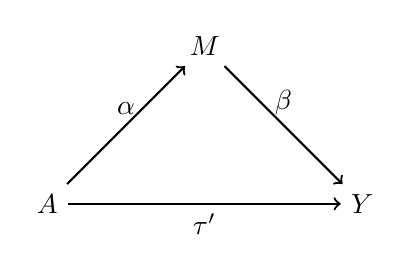
\begin{tikzpicture}[thick]
            \node (M) at (0,2) {$ M $};
            \node (A) at (-2,0) {$ A $};
            \node (Y) at (2,0) {$ Y $};
            \draw[->] (A) -- (M) node[above,midway] {$\alpha$};
            \draw[->] (A) -- (Y) node[below,midway] {$\tau^\prime$};
            \draw[->] (M) -- (Y) node[above,midway] {$\beta$};
        \end{tikzpicture}
    \end{center}
    \begin{itemize}
        \item $ \tau^\prime $: direct effect ($ A\to Y $);
        \item $ \alpha\beta $: indirect effect ($ A\to M\to Y $);
        \item $ \tau $: total effect, that is, $ \tau=\alpha\beta+\tau^\prime $;
        \item $ M $ is the \textbf{intermediate} variable.
    \end{itemize}
\end{Regular}
\begin{Regular}{Slide 8}
    \begin{align}
        Y & =\beta_1+\tau A + \varepsilon_3               \\
        Y & =\beta_2+\tau^\prime A+\beta M +\varepsilon_2 \\
        M & =\beta_3+\alpha A+\varepsilon_3
    \end{align}
    Plug in (3) into (2),
    \begin{align*}
        Y
         & =\beta_2+\tau^\prime A +\beta(\beta_3+\alpha A+\varepsilon_3)+\varepsilon_2                                                                                \\
         & =\underbrace{\beta_2+\beta\beta_3}_{\beta_1}+\underbrace{(\tau^\prime+\alpha\beta)}_{\tau}A+\underbrace{\beta\varepsilon_3+\varepsilon_2}_{\varepsilon_1},
    \end{align*}
    which yields $ \tau=\tau^\prime+\alpha\beta\implies \tau-\tau^\prime=\alpha\beta $.
    \begin{itemize}
        \item $ \tau-\tau^\prime $: subtraction approach.
        \item $ \alpha\beta $: product approach.
    \end{itemize}
\end{Regular}
\begin{Regular}{Slide 10}
    Why can the direct and indirect effect be opposite? (for the following diagram)
    \begin{center}
        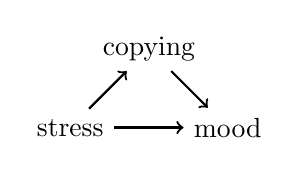
\begin{tikzpicture}[thick]
            \node (M) at (0,1) {copying};
            \node (A) at (-1,0) {stress};
            \node (Y) at (1,0) {mood};
            \draw[->] (M) to (Y);
            \draw[->] (A) to (Y);
            \draw[->] (A) to (M);
        \end{tikzpicture}
    \end{center}
\end{Regular}
\begin{Regular}{Slide 11}

    When testing the mediation effect, we can conduct the following hypothesis:
    \[ \HN\colon \alpha\beta=0, \]
    which is a \emph{composite} hypothesis. That is, we will need to test
    \begin{itemize}
        \item $ \alpha=0 $, $ \beta\ne 0 $;
        \item $ \alpha\ne 0 $, $ \beta=0 $;
        \item $ \alpha=0 $, $ \beta=0 $.
    \end{itemize}
    To get the test statistic, we use the Delta method.
    \begin{itemize}
        \item $ \E{X}\approx \hat{\mu} $ is consistent;
        \item $ \Var{X}\approx \text{se}^2(X) $.
        \item To get $ \Var{g(X)} $, using the first-order Delta method, we get
              \begin{align*}
                  \Var{g(X)}
                   & \approx \bigl[g^\prime(\hat{\mu})\bigr]^2
                  \text{se}^2(X),
              \end{align*}
              assuming $ g(\:\cdot\:) $ is differentiable.
    \end{itemize}
    In the bivariate case,
    \begin{itemize}
        \item $ g(X,Y)=XY $, so that
              \[ \nabla g(X,Y)=\begin{bmatrix}
                      \pdv{g}{X} \\
                      \pdv{g}{Y}
                  \end{bmatrix}=
                  \begin{bmatrix}
                      Y \\
                      X
                  \end{bmatrix}. \]
        \item We know that
              \[ \Var{\hat{\alpha}}\approx \text{se}^2(\hat{\alpha}), \]
              \[ \Var{\hat{\beta}}\approx \text{se}^2(\hat{\beta}). \]
              Hence, using the first-order Delta method, we get
              \begin{align*}
                  \Var{\hat{\alpha}\hat{\beta}}
                   & \approx \begin{bmatrix}
                                 \hat{\beta} & \hat{\alpha}
                             \end{bmatrix}\begin{bmatrix}
                                              \text{se}^2(\hat{\alpha}) & 0                        \\
                                              0                         & \text{se}^2(\hat{\beta})
                                          \end{bmatrix}\begin{bmatrix}
                                                           \hat{\beta} \\
                                                           \hat{\alpha}
                                                       \end{bmatrix}       \\
                   & =\hat{\alpha}^2\text{se}^2(\hat{\beta})+\hat{\beta}^2\text{se}^2(\hat{\alpha}).
              \end{align*}
    \end{itemize}
\end{Regular}

\section*{Chapter 6 Part II}
\begin{Regular}{Slide 5}
    \begin{align*}
        \text{CDE}_1
         & =\E{Y^{1,1}-Y^{0,1}}                                   \\
         & =\alpha_0+\alpha_1+\alpha_2+\alpha_3-\alpha_0-\alpha_2 \\
         & =\alpha_1+\alpha_3.
    \end{align*}
\end{Regular}

\makeheading{Week 8 | Wednesday}{\printdate{2022-03-02}}%chktex 8
\begin{Regular}{Slide 3}
    \begin{center}
        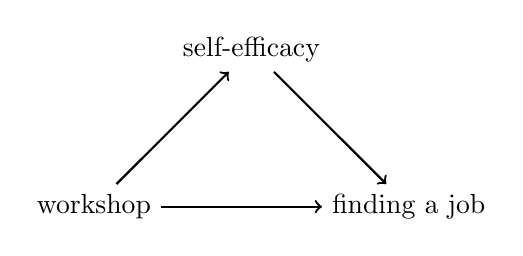
\begin{tikzpicture}[thick]
            \node (M) at (0,2) {self-efficacy};
            \node (A) at (-2,0) {workshop};
            \node (Y) at (2,0) {finding a job};
            \draw[->] (M) to (Y);
            \draw[->] (A) to (Y);
            \draw[->] (A) to (M);
        \end{tikzpicture}
    \end{center}
    If $ M $ is binary,
    \begin{itemize}
        \item $ \text{CDE}_1=\E{Y^{1,1}-Y^{0,1}} $;
        \item $ \text{CDE}_0=\E{Y^{1,0}-Y^{0,0}} $.
    \end{itemize}
    If there is no interaction between $ A $ and $ M $, then
    \[ \text{CDE}=\text{CDE}_1=\text{CDE}_0. \]
\end{Regular}
\begin{Regular}{Slide 5}
    Since we have two time points now and using the diagram
    on \textbf{slide 4}, we see that
    \begin{align*}
        sw_i
         & =sw_i(1)\times sw_i(2)                         \\
         & =\frac{\Prob{A=A_i}}{\Prob{A=A_i\given X=X_i}}
        \times \frac{\Prob{M=M_i\given A=A_i}}{\Prob{M=M_i\given A=A_i,X=X_i,W=W_i}}.
    \end{align*}
    \textbf{Slide 7}
    \begin{center}
        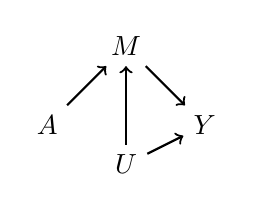
\begin{tikzpicture}[thick]
            \node (M) at (0,1) {$ M $};
            \node (A) at (-1,0) {$ A $};
            \node (Y) at (1,0) {$ Y $};
            \node (U) at (0,-0.5) {$ U $};
            \draw[->] (M) to (Y);
            \draw[->] (A) to (M);
            \draw[->] (U) to (M);
            \draw[->] (U) to (Y);
        \end{tikzpicture}
    \end{center}
    \begin{itemize}
        \item $ A $: treatment being assigned;
        \item $ M $: treatment actually received;
        \item $ Y $: outcome;
        \item $ U $: age.
    \end{itemize}
    We lose the ability to draw a causal inference between $ A $ and $ Y $.
\end{Regular}
\begin{Regular}{Slide 10}
    Using the conditional probabilities, the total effect is
    \begin{align*}
        \E{Y^1-Y^0}
         & =\text{CACE}p_C+\text{DACE}p_D
        +\text{AACE}p_A+\text{NACE}p_M.
    \end{align*}
    \begin{itemize}
        \item The exclusion restriction implies
              $ \text{AACE}=\text{NACE}=0 $.
        \item The monotocity assumption implies $ p_D=0 $.
        \item The third assumption implies
              $ \E{Y^1-Y^0}=\E{Y\given A=1}-\E{Y\given A=0} $.
    \end{itemize}
    Re-arranging,
    \[ \widehat{\text{CACE}}=\frac{\estE{Y^1-Y^0}}{\hat{p}_C}
        =\frac{\estE{Y\given A=1}-\estE{Y\given A=0}}{\hat{p}_C}. \]
    Looking at the quantity
    \[ \Prob{M=1\given A=1}-\Prob{M=1\given A=0}, \]
    we see that
    \begin{itemize}
        \item $ \Prob{M=1\given A=1} $ are the always takers and compliers, and
        \item $ \Prob{M=1\given A=0} $ are the always takers (and defiers; although
              there is no defiers in this case).
    \end{itemize}
    Hence,
    \[ \hat{p}_C=\estE{M\given A=1}-\estE{M\given A=0}, \]
    which yields the same formula for $ \widehat{\text{CACE}} $ as \textbf{slide 11}.
\end{Regular}
\begin{Regular}{Slide 18}
    If $ A_i=1 $, we need to first impute $ M_i^0 $ with
    \[ M \sim A+X, \]
    and then impute
    $ Y_i^{1,M_i^0} $, $ Y_i^{0,M_i^1} $, $ Y_i^{0,M_i^0} $
    with
    \[ Y \sim M+A+X. \]
\end{Regular}
\section*{Case Study III\@: Mediation Analysis}
\begin{Regular}{Slide 6}
    The output line-by-line is:
    \begin{itemize}
        \item $ \text{NIE}_0 $;
        \item $ \text{NIE}_1 $;
        \item $ \text{NDE}_0 $;
        \item $ \text{NDE}_1 $;
        \item $ \text{TE} $;
        \item $ \text{NIE}_0/\text{TE} $;
        \item $ \text{NIE}_1/\text{TE} $,
    \end{itemize}
    and rest are unimportant.
\end{Regular}